\documentclass[12pt,a4paper]{article}

\usepackage{xeCJK}
\usepackage{amsmath,amsthm,amssymb}
\usepackage{hyperref}
\usepackage{graphicx}
\usepackage{tikz}
\usepackage{xcolor}
\usepackage{float}
\usepackage{makeidx}
\usepackage{listings} 
\usepackage[numbers,sort&compress]{natbib}
\usepackage[level]{datetime}
\usepackage[top=1.5cm, bottom=2cm, outer=1.5cm, inner=1.5cm, heightrounded, marginparwidth=0cm, marginparsep=0cm]{geometry}
%\usepackage{showframe}

\renewcommand{\today}{\number\year 年 \number\month 月 \number\day 日}
\renewcommand{\refname}{参考文献}
\renewcommand{\tablename}{表}
\renewcommand{\contentsname}{目录}

\newcommand{\upcite}[1]{\textsuperscript{\textsuperscript{\cite{#1}}}}
\newcommand{\tabincell}[2]{\begin{tabular}{@{}#1@{}}#2\end{tabular}}

\definecolor{dkgreen}{rgb}{0,0.6,0}
\definecolor{gray}{rgb}{0.5,0.5,0.5}
\definecolor{mauve}{rgb}{0.58,0,0.82}
\lstset{
  language=c++, 
  basicstyle=\footnotesize,  
  % numbers=left,      
  numberstyle=\tiny\color{gray}, 
  stepnumber=2, 
  numbersep=5pt,
  backgroundcolor={},
  showspaces=false,   
  showstringspaces=false,
  showtabs=false,         
  frame=single,                   % frame around code [single, shadowbox]
  rulecolor=\color{black}, 
  tabsize=2,                     
  captionpos=b,                   % caption-position bottom
  breaklines=true,                % automatic line breaking
  breakatwhitespace=false, 
  % title=\lstname,               % filename included with \lstinputlisting;
  keywordstyle=\color{blue},     
  commentstyle=\color{dkgreen}, 
  stringstyle=\color{mauve},     
  escapeinside={\%*}{*)},         % if want to add LaTeX within your code
  morekeywords={*,...}            % if want to add more keywords to the set
}

\title{第四节课习题}
\author{高洪臣}
\date{2019年7月12日}

\begin{document}

\maketitle

\noindent
\setlength{\parindent}{2em}
\setlength{\parskip}{0.3em}
\linespread{1}

\section*{基础题} 

\begin{enumerate}

\item 完成单目 Bundle Adjustment 求解器 problem.cc 中的部分代码


\begin{itemize}

\item 完成 Problem::MakeHessian() 中信息矩阵 H 的计算

\begin{lstlisting}
// 按照代码顺序
// part 1
H.block(index_i, index_j, dim_i, dim_j).noalias() += hessian;
// part 2
H.block(index_j, index_i, dim_j, dim_i).noalias() += hessian.transpose();
\end{lstlisting}

\item 完成 Problem::SolveLinearSystem() 中 SLAM 问题的求解

\begin{lstlisting}
// 按照代码顺序
// part 1
MatXX Hmm = Hessian_.block(reserve_size,reserve_size,marg_size,marg_size);
MatXX Hpm = Hessian_.block(0,reserve_size,reserve_size,marg_size);
MatXX Hmp = Hessian_.block(reserve_size,0,marg_size,reserve_size);
VecX bpp = b_.segment(0,reserve_size);
VecX bmm = b_.segment(reserve_size,marg_size);
// part 2 
H_pp_schur_ = Hessian_.block(0,0,reserve_size,reserve_size)-tempH*Hmp;
b_pp_schur_ = bpp - tempH * bmm;
// part 3
delta_x_ll = Hmm_inv * (bmm - Hmp * delta_x_pp);
\end{lstlisting}

\end{itemize}


\item 完成滑动窗口算法测试函数

\begin{itemize}
\item 完成 Problem::TestMarginalize() 中的代码,并通过测试
\begin{lstlisting}
// 按照代码顺序
// part 1
H_marg.block(idx, 0, reserve_size - idx - dim, reserve_size) = temp_botRows;
H_marg.block(reserve_size - dim, 0, dim, reserve_size) = temp_rows;
// part 2
Eigen::MatrixXd Arm = H_marg.block(0, n2, n2, m2);
Eigen::MatrixXd Amr = H_marg.block(n2, 0, m2, n2);
Eigen::MatrixXd Arr = H_marg.block(0,  0, n2, n2);
\end{lstlisting}
\end{itemize}


\item 运行结果(完整工程代码见 \textbf{code} 文件夹)

\begin{figure}[htbp] 
	\centering
	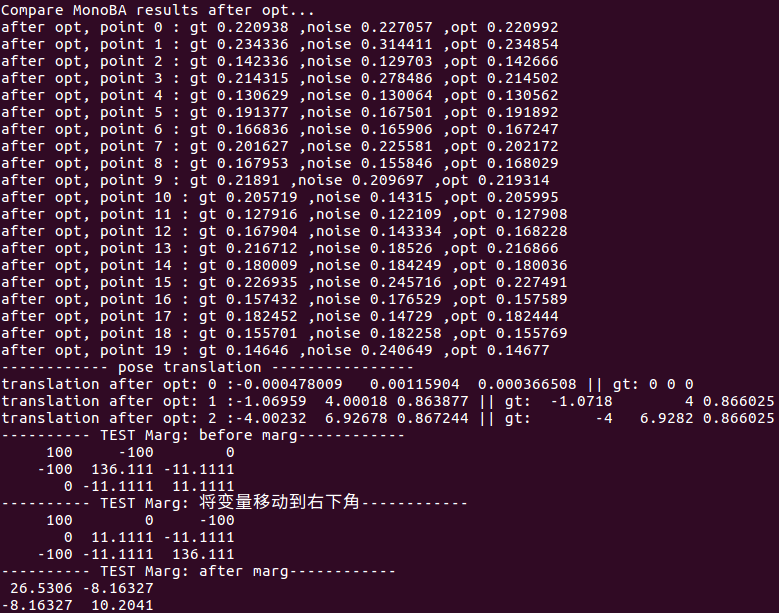
\includegraphics[width=15cm]{ba_mono_01.png}
	\caption{没有 fix 第一帧和第二帧}
\end{figure} 

\begin{figure}[htbp] 
	\centering
	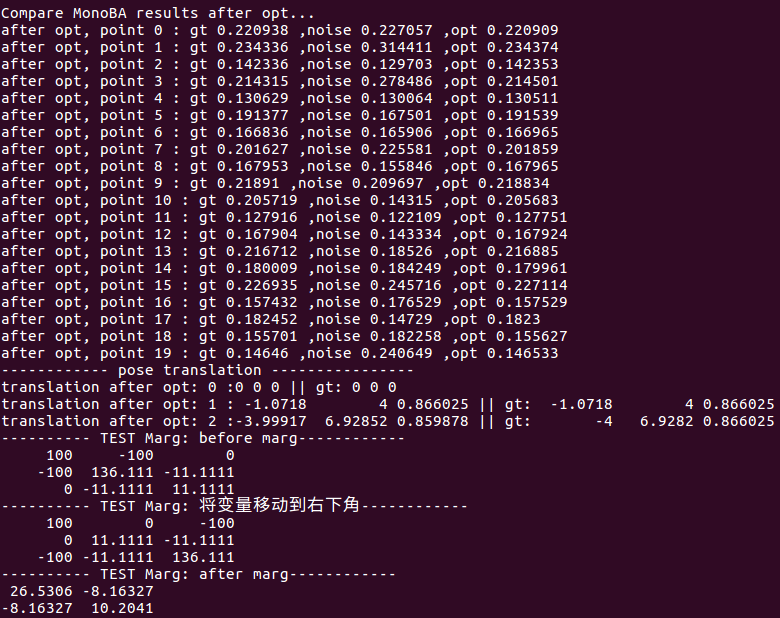
\includegraphics[width=15cm]{ba_mono_02.png}
	\caption{fix 第一帧和第二帧}
\end{figure} 

\end{enumerate}


\newpage

\section*{提升题}

paper reading~\cite{zhang2018comparison},请总结论文:优化过程中处理 H 自由度的不同操作方式。总结内容包括:具体处理方式,实验效果,结论。\newline

答:  

单目VO有7个不可观的自由度(双目VO有6个),VIO有4个不可观的自由度(全局位置和yaw不可观测),称为\textbf{规范自由度(gauge freedom)}。

VIO优化时,需要特别处理这4个自由度,通常有三种方法:固定这四个自由度、给这四个自由度加先验、任意优化这四个自由度最后reset。

\begin{enumerate}

\item 具体处理方式

\begin{figure}[htbp] 
	\centering
	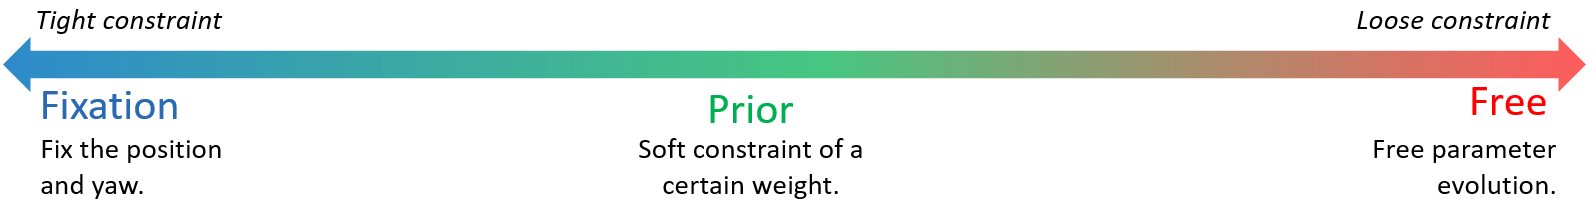
\includegraphics[width=15cm]{vio_gauge_freedom.png}
\end{figure} 

\begin{enumerate}

\item Gauge Fixation: fixing the initial state

固定第一帧相机的位置 $p_0$ 和 偏航角yaw,将其设定为常量,限制规范自由度
$$
p_0 = p_0^0, \quad \Delta \phi_{0z} = 0
$$
等价于, 对应的视觉残差的雅克比矩阵为$\mathbf{0}$
$$
J_{p_0} = \mathbf{0}, \quad J_{\Delta \phi_{0z}} = \mathbf{0}
$$

\item Gauge Prior: adding a prior to the initial state

使用合适的先验协方差矩阵 $\Sigma_0^P$,给视觉残差最小二乘添加惩罚
$$
\|r_0^P\|^2_{\Sigma_0^P}
$$
通常,
$$
\Sigma_0^P = \sigma_0^2 I
$$

\item Free Gauge: allowing the parameters to evolve freely during optimization

使用伪逆或添加阻尼项(LM)处理Hessian矩阵,然后再将所有帧重置

伪逆
$$
\Delta x = H^{+} b
$$

添加阻尼项
$$
\Delta x = (H + \mu \lambda)^{-1} b
$$

\end{enumerate}

\item 实验效果

选择合适的先验权重:
\begin{itemize}
\item Accuracy:当先验权重超过某个阈值后,估计误差的RMSE稳定在一个值
\item Computational Cost:当先验权重超过某个阈值后,迭代次数和收敛时间也会稳定
\end{itemize}

选择合适的先验权重后,\textbf{Gauge Prior}和\textbf{Gauge Fixation}的精度和计算代价几乎相同。

协方差比较:

\begin{figure}[htbp] 
	\centering
	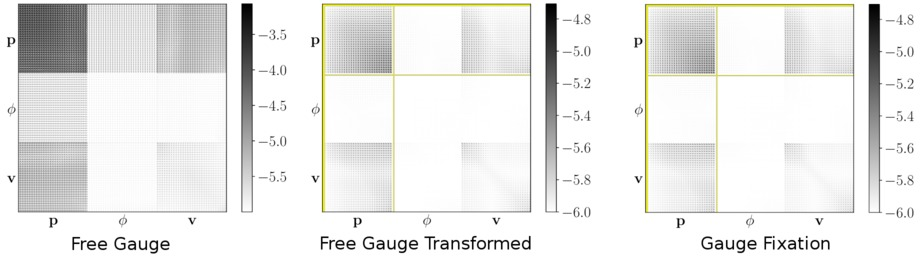
\includegraphics[width=15cm]{cov_mat.jpg}
\end{figure} 

\item 结论

\begin{itemize}
\item \textbf{Accuracy}:三种方式精度都差不多

\item \textbf{Efficiency}:\textbf{Free Gauge},即 任意优化然后reset的操作,收敛所需要的迭代次数较少,速度快一点,效率较高;不过没有一个参考系,信息矩阵的逆得到的协方差没有太多的意义;\textbf{Gauge Prior}需要选择合适的先验协方差权重,来避免计算代价的增加

\item \textbf{Covariance}:三种方式的协方差是紧密相关的,free gauge的协方差可通过线性变换变为gauge fixation的协方差
\end{itemize}

\item 代码

协方差变换的代码:\href{https://github.com/uzh-rpg/rpg_vi_cov_transformation}{rpg\_vi\_cov\_transformation} 


\end{enumerate}



\bibliographystyle{unsrt}
\bibliography{bibfile}

\end{document}

